\documentclass[titlepage=firstiscover, captions=tableheading, bibliography=totoc]{scrartcl}

\usepackage{polyglossia}
\setmainlanguage{german}

\usepackage{fontspec}
\usepackage{amsmath}
\usepackage{amssymb}
\usepackage{mathtools}
\usepackage[locale=DE, separate-uncertainty=true, per-mode=symbol-or-fraction]{siunitx}
\usepackage{microtype}
\usepackage{xfrac}
%\usepackage{subcaption}
%\usepackage{graphicx}
%\usepackage{grffile}
\usepackage{booktabs}
\usepackage{biblatex}
\addbibresource{litvz.bib}

\usepackage{lscape}

\usepackage[math-style=ISO,bold-style=ISO,sans-style=italic,nabla=upright,partial=upright,]{unicode-math}
\setmathfont{Latin Modern Math}

\begin{document}

\title{V308 Magnetfelder und Spulen}
\author{Katharina Brägelmann \and Tobias Janßen \and katharina.braegelmann@tu-dortmund.de \and tobias2.janssen@tu-dortmund.de}
\date{Durchführung: 15. Dezember 2017, Abgabe: 22. Dezember 2017}
\maketitle

\tableofcontents

%\input{lit.bib}

\newpage

\section{Zielsetzung}
\input{Zielsetzung.txt}


\section{Theorie}
\section{Zielsetzung}
Ziel des Versuches ist es das Trägheitsmoment unterschiedlicher Körper zu ermitteln.
Zusätzlich wird der Satz von Steiner verifiziert.


\section{Theorie}
Rotationsbewegungen lassen sich durch das Drehmoment M, die Winkelbeschleunigung $\dot{\omega} $ und das Trägheitsmoment I beschreiben.
Das Trägheitsmoment beschreibt die Massenverteilung eines Körpers im Bezug auf die Rotationsachse.
Das Gesamtträgheitsmoment lässt sich dabei beschreiben durch

\begin{equation*}
  I = \sum_i r_i^2 \cdot m_i.
\end{equation*}
\\$m_i$ ist dabei ein Massenelement mit dem Abstand $r_i$ zur Drehachse. Für infinitesimale Körper ergibt sich

\begin{equation*}
  I = \int r^2 dm.
\end{equation*}
\\Geht die Drehachse nicht durch den Schwerpunkt des Körpers muss das Trägheitsmoment durch den Satz von Steiner beschrieben werden:

\begin{equation}
  I = I_s + m \cdot a^2.
  \label{eqn:steiner}
\end{equation}
\\$I_s$ ist dabei das Tragheitsmoment bezüglich der Drehachse des Schwerpunktes.
Für das Drehmoment M eines Körpers auf den die Kraft F im Abstand r wirkt, gilt die Formel:

\begin{equation*}
  \vec{M} = \vec{F}\times \vec{r}.
\end{equation*}
\\Stehen F und r senkrecht zueinander gilt

\begin{equation*}
  M = F\cdot r.
\end{equation*}
\\Bei schwingenden System wirkt der Auslenkung $\phi$ ein rücktreibendes Drehmoment entgegen, welches beschrieben wird durch:

\begin{equation*}
  M = D \cdot \phi
\end{equation*}
\\mit der Winkelrichtgröße D.
\\Die Schwingungsdauer beträgt

\begin{equation}
  T = 2\pi\sqrt\frac{I}{D}.
\label{eqn:schwing}
\end{equation}
\\Die Formel gilt jedoch nur für kleine Winkel. Sie lässt sich umstellen zu
\begin{equation}
  I = \frac{T^2 \cdot D}{(2 \pi)^2}.
\label{eqn:schwing2}
\end{equation}
\\Das Trägheitsmoment I eines Zylinders, bei dem die Drehachse durch den Schwerpunkt geht und senkrecht zur Bodenfläche steht, ist das Trägheitsmoment
\begin{equation}
  I_{zs} = \frac{m \cdot R^2}{2}.
\label{eqn:Zs}
\end{equation}
\\Für einen liegenden Zylinder, bei dem die Achse durch den Schwerpunkt geht, ist das Trägheitsmoment
\begin{equation}
  I_{zl} = m \left(\frac {R^2}{4}+\frac {h^2}{12} \right).
\label{eqn:Zl}
\end{equation}
\\Ein Stab, der sich um eines seiner Enden dreht, hat das Trägheitsmoment
\begin{equation}
  I_{st} = \frac{m \cdot L^2}{3}
  \label{eqn:stab}
\end{equation}

\newpage


\section{Aufbau und Durchführung}
\subsection{Aufbau}
Der Aufbau des Experiments ist in folgender Abbildung dargestellt:
\begin{figure}[h!]
  \centering
  \includegraphics[width=\textwidth]{Aufbau.pdf}
  \caption{Schematischer Aufbau der Messapparatur}
  \label{aufbau}
\end{figure}
\\Ein Permanentmagnet ist in eine Kugel eingelassen, hier Billardkugel genannt.
Ein Messingzylinder steht in der Mitte eines Helmholtzspulenpaars mit den Abmessungen $N=195$, $d=\SI{0.138}{m}$ und $R=\SI{0.109}{m}$.
Die Billardkugel wird auf ein Luftkissen auf dem Messingzylinder gelegt.
Am Rand der oberen Helmholtzspule ist ein Stroboskoplicht angebracht.
An dem Steuergerät können die Magnetfeld-erzeugende Stromstärke an den Spulen und das Stroboskop eingestellt werden.
Außerdem wird das Luftkissen über das Steuergerät ein- und ausgeschaltet.

\subsection{Durchführung der Bestimmung des magnetischen Momentes unter Ausnutzung der Gravitation}
Für diese Methode wird eine verschiebbare Masse an einem dünnen Aluminiumstift in die Billardkugel gesteckt.
Die Masse wird als Punktmasse angesehen und die Masse des Aluminiumstiftes wird vernachlässigt.
Das Luftkissen wird eingeschaltet und die Richtung des Magnetfelds so eingestellt, dass es nach oben wirkt.
Der Radius der Masse vom Mittelpunkt der Billardkugel wird mithilfe einer Schieblehre festgelegt und die Billardkugel auf das Luftkissen gesetzt.
Dann wird der Spulenstrom so weit hochgedreht, bis die Kräfte in einem Gleichgewicht sind und die Billardkugel nicht mehr umkippt.
Der gesetzte Radius der Masse zum Mittelpunkt der Billardkugel und die Spulenstromstärke werden notiert.
Aus der Stromstärke wird das entsprechende Magnetfeld berechnet.
Die Messung wird für insgesamt 14 Radien durchgeführt.

\subsection{Durchführung der Bestimmung des magnetischen Momentes über die Schwingungsdauer des Magneten}
Bei dieser Methode wird zunächst das Luftkissen angestellt.
Die Richtung des Magnetfelds ist nach oben gehend.
Die Spulenstromstärke wird eingestellt und die Billardkugel wird auf dem Luftkissen vorsichtig ausgelenkt.
Die Schwingungsdauer von zehn Schwingungen wird gemesssen.
Daraus wird die Dauer einer Schwingung gemittelt.
Es werden die Spulenstromstärke und die gemittelte Schwingungsdauer notiert.
Die Messung wird mit 13 weiteren Stromstärken durchgeführt.

\subsection{Durchführung der Bestimmung des magnetischen Momentes über die Präzession der Billardkugel}
Es wird das Luftkissen eingeschaltet.
Das Stroboskoplicht wird auf eine Frequenz von 6Hz geregelt.
Anschließend wird die Billardkugel auf dem Luftkissen in Rotation versetzt und das Stroboskoplicht angestellt.
Sobald der weiße Punkt auf der Billardkugel als konstant, nicht mehr blinkend, wahrgenommen wird, wird die Billardkugel vorsichtig ausgelenkt und die Spulenstromstärke aufgedreht.
Die Umlaufdauer der Präzessionsbewegung wird gemessen und gemeinsam mit der Spulenstromstärke notiert.
Die Messung wird für die selbe Stromstärke drei mal wiederholt und die Umlaufzeiten gemittelt.
Die Messung wird für insgesamt zehn verschiedene Spulenstromstärken durchgeführt.

\newpage
\FloatBarrier

\section{Auswertung}
\subsection{Auswertung zu V501}


Die gemessenen Werte für die Beschleunigungsspannung $U_{B}$, die Ablenkung des Elektronenstrahls $D$ und die Ablenkspannung $U_{\text{d}}$ sind in der Tabelle
\ref{tab:V501} aufgeführt.
%\documentclass[captions=tableheading]{scrartcl}
%\usepackage{booktabs}
%\usepackage{pdflscape}




%\begin{document}
%\begin{landscape}


\begin{table}[h!]
  \centering
  \caption{Messergebnisse $U_\text{d}$ und D in Abhängigkeit von $U_B$}
  \label{tab:V501}
  \begin{tabular}{c c c c c c c c c c}
    \toprule
    \multicolumn{2}{c}{$U_B = 150V $} &   \multicolumn{2}{c}{$U_B = 250V$}&    \multicolumn{2}{c}{$U_B = 350V$}& \multicolumn{2}{c}{$U_B = 450V$}&  \multicolumn{2}{c}{$U_B = 480$}\\
      \midrule
    $U_\text{d}$ & $\text{D}$ & $U_\text{d}$ & $\text{D}$ & $U_\text{d}$ & $\text{D}$ & $U_\text{d}$ & $\text{D}$ & $U_\text{d}$ & $\text{D}$\\
      V &     cm &   V &     cm &   V &    cm  &  V  &  cm    &  V  & cm \\
    \midrule

    -7,3&			 1,5875& -12,3	&				 1,524& 16,4&					 1,4478 & -19,7&					 1,3462 & -&-\\
    -4,5&			 0,9525& -7,5 	&				 0,889& 10,5&					 0,8128 & -11,3&					 0,7112 & -10,6&					 0,635\\
    -1,6&			 0,3175& -2,7 	&				 0,254& -3,7&					 0,1778 &   -2,9&					 0,0762 &   -0,9&					 0,0\\
     1,1&			-0,3175&  2,4	  &				-0,381&  2,9&					-0,4572 &    6,4&					-0,5588 &    8,6&					-0,635\\
     3,6&			-0,9525&  6,9	  &				-1,016&  9,8&					-1,0922 &   13,6&					-1,1938 &   17,9&					-1,27\\
     6,2&			-1,5875& 11,4	  &				-1,651& 15,7&					-1,7272 &   21,6&					-1,8288 &   27,0&					-1,905\\
     8,8&			-2,2225& 16,2	  &				-2,286& 22,6&					-2,3622 &   29,6&					-2,4638 & -     &-           \\
     11,4&		-2,8575& 20,8	  &				-2,921& 28,8&					-2,9972 &      -&            -    &   -    & -     \\
     14,0&		-3,4925& 25,6	  &				-3,556& 34,4&					-3,6322 &     - &             -   &    -   &-      \\
    \bottomrule
  \end{tabular}
\end{table}

%\end{landscape}
%\end{document}

In den Abbildungen \ref{fig:150V}, \ref{fig:250V}, \ref{fig:350V}, \ref{fig:450V} und \ref{fig:480V} wird $D$ gegen $U_{\text{d}}$ aufgetragen.

\begin{figure}[h!]
  \centering
  \includegraphics[width=0.8\textwidth]{150V.pdf}
  \caption{Höhe D gegen $U_{\text{d}} f\ddot{u}r 150V$}
  \label{fig:150V}
\end{figure}

\begin{figure}[h!]
 \centering
 \includegraphics[width=0.8\textwidth]{250V.pdf}
 \caption{Höhe D gegen $U_{\text{d}} f\ddot{u}r 250V$}
 \label{fig:250V}
\end{figure}

\begin{figure}[h!]
  \centering
  \includegraphics[width=0.8\textwidth]{350V.pdf}
  \caption{Höhe D gegen $U_{\text{d}} f\ddot{u}r 350V$}
  \label{fig:350V}
\end{figure}

\begin{figure}[h!]
  \centering
  \includegraphics[width=0.8\textwidth]{450V.pdf}
  \caption{Höhe D gegen $U_{\text{d}} f\ddot{u}r 450V$}
  \label{fig:450V}
\end{figure}

\begin{figure}[h!]
  \centering
  \includegraphics[width=0.8\textwidth]{480V.pdf}
  \caption{Höhe D gegen $U_{\text{d}}  f\ddot{u}r  480V$}
  \label{fig:480V}
\end{figure}
\begin{align*}
  150V\\
  Steigung:   (-0.24155702\pm6.70315714\cdot10^{-6})\si{\frac{cm}{V}}\\
  Y-Achse:    (-0.11241836\pm3.89639666\cdot10^{-4})\si{cm}
\end{align*}


\begin{align*}
  250V\\
  Steigung: (-0.13446489\pm4.13337095\cdot10^{-7})\si{\frac{cm}{V}}\\
  Y-Achse:  (-0.10761495\pm8.03068033\cdot10^{-5})\si{cm}
\end{align*}


\begin{align*}
350V\\
Stiegung: (-0.09853167\pm6.37684729\cdot10^{-7})\si{\frac{cm}{V}}\\
Y-Achse:  (-0.17695027\pm2.31507889\cdot10^{-4})\si{cm}
\end{align*}

\begin{align*}
450V\\
Steigung: (-0.07717596\pm9.45031190\cdot10^{-7})\si{\frac{cm}{V}}\\
Y-Achse:  (-0.14756239\pm2.82541359\cdot10^{-4})\si{cm}
\end{align*}

\begin{align*}
480V\\
Steigung: (-0.06754249\pm2.40937941\cdot10^{-7})\si{\frac{cm}{V}}\\
Y-Achse:  (-0.06764309\pm5.95858844\cdot10^{-5})\si{cm}
\end{align*}

Mit Hilfe einer von Phyton errechneten Ausgleichsgraden kann die Empfindlichkeit $D/U_\text{d}$ für die verschiedenen Beschleunigungsspannungen ermittelt werden.
Die ermittelte Empfindlichkeit wird nun gegen $1/U_B$ aufgetragen und eine Ausgleichsrechnung durchgeführt. Dies ist in der Abbildung \ref{fig:Ergebniss} zu sehen.
\begin{figure}[h!]
  \centering
  \includegraphics[width=0.8\textwidth]{Ergebniss.pdf}
  \caption{$D/U_{\text{d}}$ gegen $1/U_B$}
  \label{fig:Ergebniss}
\end{figure}
\\Die Steigung der Ausgleichsgraden beträgt:
\begin{equation*}
  a=\SI{0,3730 \pm 0,0115}{m}
\end{equation*}
\begin{align*}
  p=\SI{0,019}{m}\\
  d=\SI{0,0038}{m}\\
  L=\SI{0,1533}{m}\\
  \frac{pL}{2d}=\SI{0,38325}{m}
\end{align*}
\\Nun wird die Frequenz der Sinusspannung bestimmt. Als Beschleunigungsspannung wird $U_B=\SI{280}{V}$ verwendet.
Für bestimmte Frequenzen zeigt das Oszilloskop stehende Wellen an. Diese Frequenzen sind in der Tabelle \ref{tab:Frequenz} aufgeführt.
Der gemittelte Wert für $\nu_{\text{sin}}$ beträgt:
\begin{align*}
  \nu_{\text{sin}}=\SI{75,146}{Hz}.
\end{align*}
Die Amplitude der Sinusfrequenz beträgt ein Kästchen auf dem Gitternetz, das sind $D = \SI{0,635}{cm}$
Die Empfindlichkeit für $U_B=\SI{280}{V}$ wird über die Ausgleichsgrade in Abbildung \ref{fig:Ergebniss} ermittelt.
%\documentclass[captions=tableheading]{scrartcl}
%\usepackage{booktabs}
%\usepackage{pdflscape}


%\begin{document}
%\begin{landscape}




\begin{table}
  \centering
  \caption{Messdaten}
  \label{tab:Frequenz}
  \begin{tabular}{c c c}
    \toprule
    $n$ & $v/Hz$ & $v/Hz$\\

    \midrule
    3     &25     & 75\\
    1,5   &50,35  & 75\\
    1     &75,24  & 75\\
    0,75  &100,35 & 75\\
    0,6   &125,36 & 75\\
    0,5   &150,95 & 75\\
    0,4   &176,9  & 75\\
    \bottomrule
  \end{tabular}
\end{table}

%\end{landscape}
%\end{document}

\begin{align*}
  \frac{D_{\text{max}}}{U_{\text{sin}}}=\SI{0,1241}{\frac{cm}{V}}\\
  U_{\text{sin}} = \SI{5,1184}{V}
\end{align*}
\FloatBarrier
\subsection{Auswertung zu V502}
Das im Experiment verwendete Helmholtz-Spulenpaar hatte einen Radius von $R = \SI{0,282}{m}$ und $N=20$ Windungen.
In der Tabelle \ref{tab:V502} ist das aus der Stromstärke errechnete B-Feld für die gemessenen Spannungen und die Größe $\frac{D}{(D^2+L^2)}$ eingetragen. L ist dabei \SI{0,1533}{m}.
%\documentclass[captions=tableheading]{scrartcl}
%\usepackage{booktabs}
%\usepackage{pdflscape}




%\begin{document}
%\begin{landscape}


\begin{table}[h!]
  \centering
  \caption{Messergebnisse der Größen $D$ und $B$ für verschiedene $U_B$}
  \label{tab:V502}
  \begin{tabular}{c c c c c c c}
    \toprule
    D & $D/(D^2+L^2)$ & $B_{250}$ & $B_{300}$ & $B_{350}$ & $B_{400}$ & $B_{440}$\\
    m & 1/m &   mT &     mT &    mT &     mT &    mT   \\
    \midrule
    0,0 &     0,0		    &  0,0     & 0,0    & 0,0    & 0,0    & 0,0   \\
    0,00635 &   0,2697    &  0,0204  & 0,0223 & 0,0223 & 0,0255 & 0,0242\\
    0,01270 &   0,5367		&  0,0408  & 0,0446 & 0,0466 & 0,0510 & 0,0510\\
    0,01905 &   0,7983		&  0,0638  & 0,0669 & 0,0701 & 0,0772 & 0,0797\\
    0,02540 &   1,0519		&  0,0816  & 0,0893 & 0,0957 & 0,1033 & 0,1084\\
    0,03175 &   1,2954		&  0,1020  & 0,1148 & 0,1116 & 0,1282 & 0,1352\\
    0,03810 &   1,5269		&  0,1224  & 0,1339 & 0,1441 & 0,1562 & 0,1652\\
    0,04445 &   1,7447		&  0,1454  & 0,1594 & 0,1690 & 0,1817 & 0,1945\\
    0,05080 &   1,9477		&  0,1658  & 0,1817 & 0,1932 & 0,2073 &       \\












    \bottomrule
  \end{tabular}
\end{table}

%\end{landscape}
%\end{document}

Trägt man die Werte in Graphen ein und führt mit Python eine Ausgleichsrechnung durch, ergiben sich die Abbildungen  \ref{fig:1-250V}, \ref{fig:1-300V}, \ref{fig:1-350V}, \ref{fig:1-400V} und \ref{fig:1-450V}.
\begin{align*}
  m_{250V} =& \SI{11844,857\pm60,887}{\frac{1}{Tm}}\\
  Y_{250V} =& \SI{0,04214751\pm0,0005875}{m}\\
  m_{300V} =& \SI{10760,858\pm48,438}{\frac{1}{Tm}}\\
  Y_{300V} =& \SI{0,04691744\pm0,00056241}{m}\\
  m_{350V} =& \SI{10107,370\pm88,829}{\frac{1}{Tm}}\\
  Y_{350V} =& \SI{0,0615518\pm0,00114344}{m}\\
  m_{400V} =& \SI{ 9421,877\pm30,996}{\frac{1}{Tm}}\\
  Y_{400V} =& \SI{0,04504514\pm0,0004708}{m}\\
  m_{450V} =& \SI{ 8946,296\pm44,868}{\frac{1}{Tm}}\\
  Y_{450V} =& \SI{0,05506224\pm0,0005871}{m}
\end{align*}
\FloatBarrier
%\begin{figure}[h!]
%  \centering
%  \includegraphics[width=0.8\textwidth]{V502.pdf}
%  \caption{$D/(D^2+L^2)$ gegen $B-Feld$}
%  \label{fig:V502}
%\end{figure}
\begin{figure}[h!]
 \centering
 \includegraphics[width=0.8\textwidth]{1-250V.pdf}
 \caption{$D/(D^2+L^2)$ gegen $B-Feld f\ddot{u}r 250V$}
 \label{fig:1-250V}
\end{figure}
\begin{figure}[h!]
 \centering
 \includegraphics[width=0.8\textwidth]{1-300V.pdf}
 \caption{$D/(D^2+L^2)$ gegen $B-Feld f\ddot{u}r 300V$}
 \label{fig:1-300V}
\end{figure}
\begin{figure}[h!]
 \centering
 \includegraphics[width=0.8\textwidth]{1-350V.pdf}
 \caption{$D/(D^2+L^2)$ gegen $B-Feld f\ddot{u}r 350V$}
 \label{fig:1-350V}
\end{figure}
\begin{figure}[h!]
 \centering
 \includegraphics[width=0.8\textwidth]{1-400V.pdf}
 \caption{$D/(D^2+L^2)$ gegen $B-Feld f\ddot{u}r 400V$}
 \label{fig:1-400V}
\end{figure}
\begin{figure}[h!]
 \centering
 \includegraphics[width=0.8\textwidth]{1-450V.pdf}
 \caption{$D/(D^2+L^2)$ gegen $B-Feld f\ddot{u}r 450V$}
 \label{fig:1-450V}
\end{figure}
Aus den Graphiken werden folgende Steigungen und Y-Achsenabschnitte errechnet.
\\Mit den Steigungen lässt sich über die Gleichung \ref{eqn:e0m0} die Konstante $\frac{e_0}{m_0}$ bestimmen.
\FloatBarrier
Der Mittelwert liegt in etwa bei $\SI{2,82070789680e11}{\frac{C}{kg}}$
\begin{align*}
  U=&250V\\
  \frac{e_0}{m_0} =& \SI{2,806012747e11}{\frac{C}{kg}}\\
  U=&300V\\
  \frac{e_0}{m_0} =& \SI{2,779105558e11}{\frac{C}{kg}}\\
  U=&350V\\
  \frac{e_0}{m_0} =& \SI{2,860449993e11}{\frac{C}{kg}}\\
  U=&400V\\
  \frac{e_0}{m_0} =& \SI{2,840696519e11}{\frac{C}{kg}}\\
  U=&440V\\
  \frac{e_0}{m_0} =& \SI{2,817274667e11}{\frac{C}{kg}}\\
\end{align*}
Für die Berechnung des Erdmagnetfeldes werden die Werte
\begin{align*}
  I =\SI{ 0,26}{A}\\
  \varphi = \SI{72}{°}
\end{align*}
\\aufgenommen.
Mit den Formeln \ref{eqn:bhor} und \ref{eqn:btot} kann das totale Erdmagnetfeld berechnet werden:
\begin{equation*}
  B = \SI{0,053}{mT}.
\end{equation*}
\FloatBarrier

\newpage
\FloatBarrier

\section{Diskussion}
Initial lässt sich sagen, dass der Versuch keine großen Abweichungen zu dem erwarteten Ergebnissen aufweist.
\\Für die erste Messung, in der der Innenwiderstand $R_{i}$ und die Leerlaufspannung $U_{0}$ der Monozelle gemessen wird, ergeben sich folgende Messwerte:
\begin{align*}
  U_{0, Mono., theo} &= \SI{1.4}{V}\\
  R_{i} &= \SI{5.05722 \pm 0.00003}{\symup\Omega}\\
  U_{0, Mono1, exp} &= \SI{1.34431 \pm 0.00006}{V}.
\end{align*}
\\Die Abweichung zwischen der initial gemessenen Leerlaufspannung und der Leerlaufspannung aus Abbildung \ref{fig:Mono} sind \SI{4.14}\%.
\\Der systematische Fehler der initialen $U_{0}$-Messung ergibt sich zu
\begin{equation*}
  \Delta U_{0}=\frac{R_{i}}{R_{V}}=\SI{7.080108e-7}{V}.
\end{equation*}
\\Die Messung der Monozelle mit der Gegenspannungsmethode liefert diesen Innenwiderstand und Leerlaufspannung:
\begin{align*}
  U_{0, Mono., theo} &= \SI{1.4}{V}\\
  R_{i} &= \SI{529.614 \pm 0.101}{\symup\Omega}\\
  U_{0, Mono2, exp} &= \SI{1.443676 \pm 0.000113}{V}.
\end{align*}
\\Die Abweichung der theoretischen Leerlaufspannung und der aus Abbildung \ref{fig:Gegen} entnommenen Leerlaufspannung liegt bei \SI{3.12}\%.
\\Die Ergebnisse der Messung mit der angelegten Rechteckspannung lassen sich zusammenfassen zu:
\begin{align*}
  U_{0, Rechteck, theo} &=\SI{0.5}{V}\\
  R_{i} &= \SI{58.67 \pm 0.002}{\symup\Omega}\\
  U_{0, Rechteck, exp} &=\SI{0.497020 \pm 0.000018}{V}.
\end{align*}
\\Die Abweichung der theoretischen und der experimentellen Leerlaufspannung beläuft sich auf \SI{0.60}\%
\\Die Ergebisse der Messung zur angelegten Sinusspannung sind:
\begin{align*}
  U_{0, Sinus, theo} &=\SI{0.67}{V}\\
  R_{i} &= \SI{690.29 \pm 0.05}{\symup\Omega}\\
  U_{0, Sinus, exp} &=\SI{0.658594 \pm 0.000004}{V}.
\end{align*}
\\Die Abweichung der initial gemessenen theoretischen Leerlaufspannung und der experimentellen Leerlaufspannung aus der Abbildung \ref{fig:Sin} ergibt sich zu \SI{1.73}\%.
\\Die geringen Abweichungen lassen sich zum Beispiel durch parallaxe Fehler, prozentuale Messfehler der Geräte und durch systematische Fehler erklären.
Der systematische Fehler durch das hochohmige Voltmeter wird nur für die Monozelle ausgerechnet, aber ähnliche Fehler sind in allen Messreihen vorhanden.
\\Die gemessene Leistung $N(R_{a})$ in Abbildung \ref{fig:Leistung} weicht systematisch von der Theoriekurve ab.
Die systematische Abweichung lässt sich unter anderem durch den Fehler der Leerlaufspannung erklären.


\FloatBarrier



\nocite{*}
\printbibliography

\begin{figure}
  \centering
  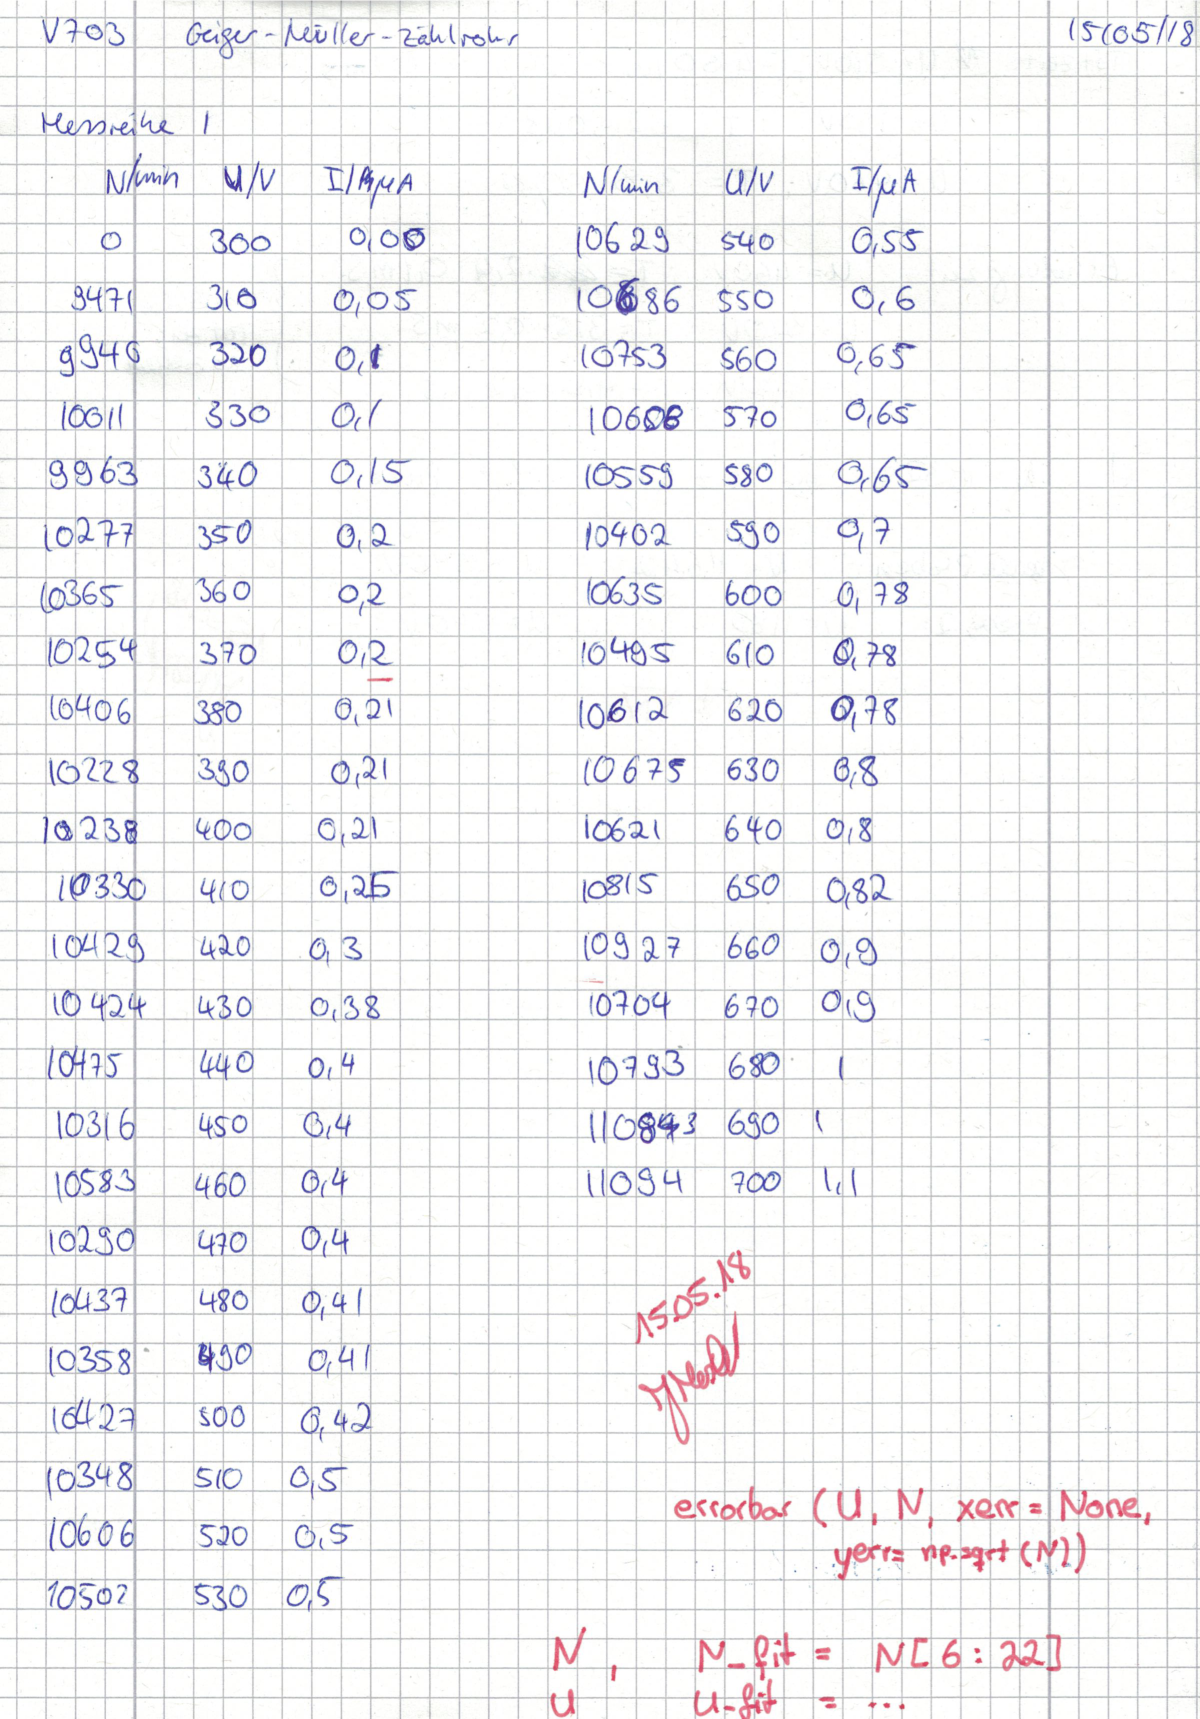
\includegraphics[width=\textwidth]{OMD1.pdf}
  \caption{Originale Messdaten}
  \label{OMD}
\end{figure}

\begin{figure}
  \centering
  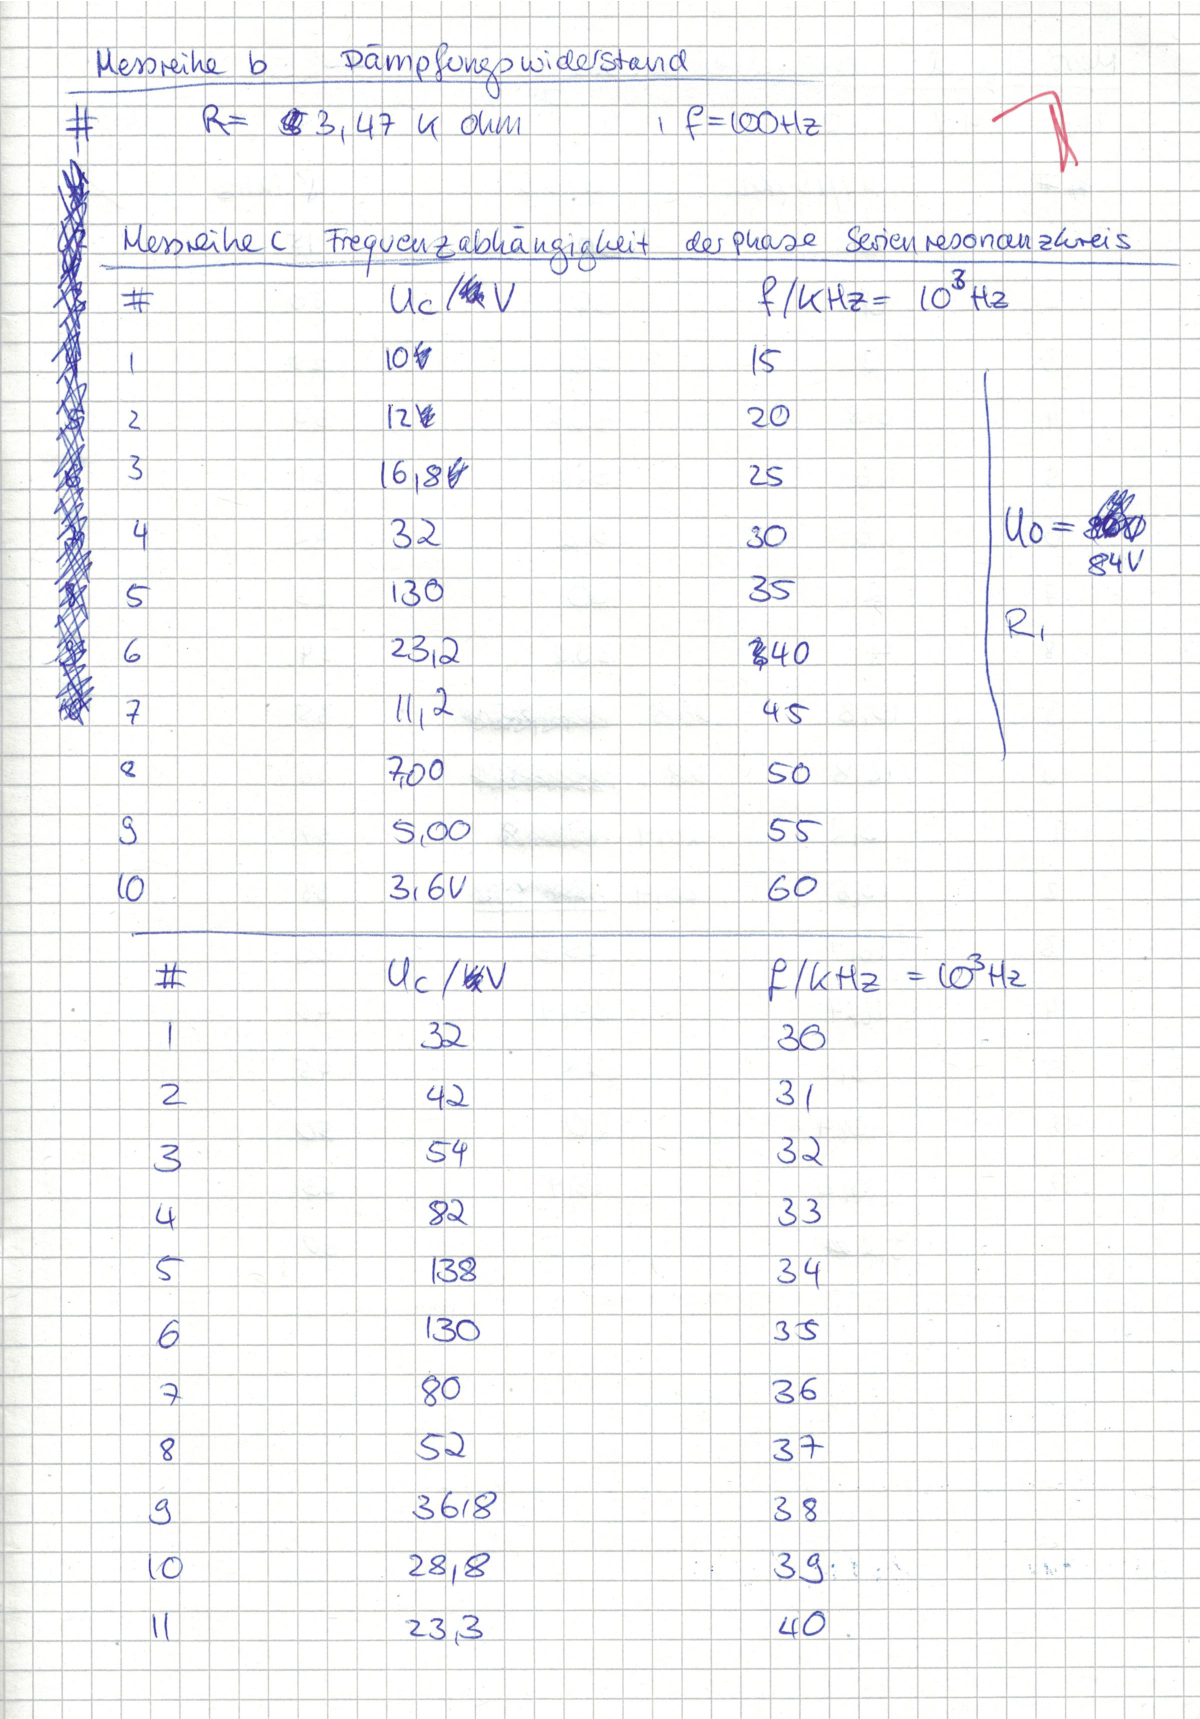
\includegraphics[width=\textwidth]{OMD2.pdf}
  \caption{Originale Messdaten}
  \label{OMD}
\end{figure}

\newpage

\end{document}
